\subsubsection{Dashboard}

\begin{center}
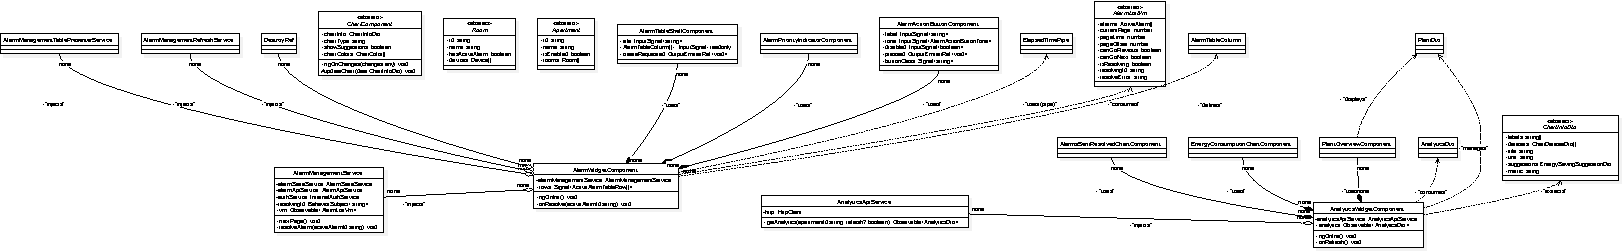
\includegraphics[width=\textwidth]{./frontend/dashboard/dashboard.pdf}
\captionof{figure}{\href{https://snakebyteteam.github.io/3-PB/Documenti_esterni/Specifica_tecnica/frontend/dashboard/dashboard.pdf}{Diagramma delle classi del modulo Dashboard}}
\end{center}


\addAtr{-}{alarmManagementService: AlarmManagementService}{}
\addAtr{-}{tablePresenter: AlarmManagementTablePresenterService}{}
\addAtr{-}{alarmManagementRefreshService: AlarmManagementRefreshService}{}
\addAtr{-}{destroyRef: DestroyRef}{}
\addAtr{+}{columns: readonly AlarmTableColumn[]}{}
\addAtr{+}{vm: Signal$<$AlarmListVm $|$ null$>$}{}
\addAtr{+}{rows: Signal$<$ActiveAlarmTableRow[]$>$}{}
\addAtr{+}{canGoPrevious: Signal$<$boolean$>$}{}
\addAtr{+}{canGoNext: Signal$<$boolean$>$}{}
\addAtr{+}{currentPage: Signal$<$number$>$}{}
\addMet{+}{ngOnInit() : void}{Inizializza il servizio di gestione allarmi e sottoscrive le notifiche di refresh per reinizializzare i dati.}
\addMet{+}{onResolve(activeAlarmId: string) : void}{Delega al servizio di gestione la risoluzione dell'allarme con l'identificativo specificato.}
\makeCl{AlarmWidgetComponent}{Componente Angular che rappresenta il widget degli allarmi attivi nella dashboard, con supporto alla paginazione e alla risoluzione. Si aggiorna automaticamente in risposta alle notifiche di refresh provenienti dal servizio dedicato.}

\addAtr{-}{refreshTrigger\$: BehaviorSubject$<$boolean$>$}{}
\addAtr{-}{analyticsApiService: AnalyticsApiService}{}
\addAtr{-}{loadTrigger\$: BehaviorSubject$<$\{id: string, refresh: boolean\} $|$ null$>$}{}
\addAtr{+}{selectedApartment\$: Observable$<$PlantDto $|$ undefined$>$ $|$ null}{}
\addAtr{+}{selectedApartmentId\$: BehaviorSubject$<$string $|$ null$>$}{}
\addAtr{+}{apartments\$: Observable$<$PlantDto[]$>$ $|$ null}{}
\addAtr{+}{analytics: Observable$<$AnalyticsDto $|$ null$>$ $|$ null}{}
\addMet{+}{ngOnInit() : void}{Inizializza il caricamento degli appartamenti, seleziona il primo disponibile e configura gli stream reattivi per l'appartamento selezionato e i dati analitici.}
\addMet{+}{getChartByMetric(data: AnalyticsDto $|$ null, metric: string) : \\ ChartInfoDto $|$ undefined}{Restituisce il grafico corrispondente alla metrica specificata dai dati analitici, o undefined se non trovato.}
\addMet{+}{onApartmentChange(event: Event) : void}{Aggiorna l'appartamento selezionato e innesca il caricamento dei relativi dati analitici.}
\addMet{+}{onRefresh() : void}{Innesca il ricaricamento forzato dei dati analitici per l'appartamento correntemente selezionato.}
\makeCl{AnalyticsWidgetComponent}{Componente Angular che rappresenta il widget di analisi nella dashboard, con supporto alla selezione dell'appartamento e al caricamento dei dati analitici. Gestisce gli stream reattivi per l'appartamento selezionato, i grafici e il refresh manuale dei dati.}

\addAtr{+}{apartment: PlantDto $|$ null}{}
\makeCl{PlantOverviewComponent}{Componente Angular che visualizza una panoramica delle informazioni di un impianto. Riceve i dati dell'impianto tramite input e li presenta nel template dedicato.}